\documentclass[tikz]{standalone}
%\usetikzlibrary{calc}
\usetikzlibrary{shapes,snakes}

\begin{document}

\tikzstyle{decision} = [diamond, draw, 
    text width=4.5em, text badly centered, node distance=3cm, inner sep=0pt]


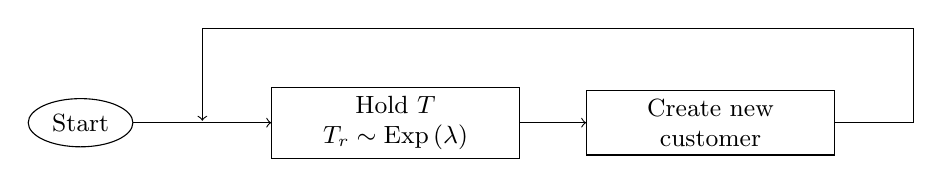
\begin{tikzpicture} [node distance=3cm, terminal/.style={ellipse, draw, text badly centered}, block/.style={rectangle, draw, text badly centered}]
{\small
  %% Customer Generator
  %\node (title) {Customer generator process};
  \node [terminal, ] (start) {Start};
  \node [block, right of=start, text width=9em, node distance=4cm] (wait) {Hold $T$\\ $T_r \sim \mathrm{Exp}\left(\lambda\right)$};
  \node [block, right of=wait, text width=9em, node distance=4cm] (create) {Create new customer};
  % Draw edges
  \draw [->] (start) -- node[midway,inner sep=0pt] (loop) {} (wait);
  \draw [->] (wait) -- (create);
  \draw [->] (create.east) -- ++(1cm, 0) -- ++(0cm, 1.2cm) -| (loop);
}
\end{tikzpicture}
\end{document}
